\section{Introduktion til Occupancy Grid}
Til at kortlægge rummet robotten befinder sig i, har vi valgt at bruge \textit{occupancy grid}.
Teorien bag denne algoritme vil blive beskrevet i dette afsnit

\section{Overblik}
Den overordnede tanke bag et occupancy grid er, at lave en ensartet inddeling af sit kort, hvor hver enkelt celle er repræsenteret af en binær \textit{stokastisk variabel}, der fortæller om den pågældende celle er 'optaget' eller ej, hvor optaget betegnes som sandsynligheden $\mathcal{P}(occupied) = 1$.
Til at begynde med initialiseres hver enkelt celle med værdien $\mathcal{P}(occupied) = 0,5$ som en indikation på, at den aktuelle tilstand endnu ikke er kendt.

En 'ledig' celle har således værdien $\mathcal{P}(occupied) = 0$.
En simpel illustration af et occupancy grid map for det kørselsmiljø, der er opstillet for vores robot, kan ses på \cref{map:approx_occupancy_grid}.

\begin{figure}[h] % Kørselsmiljø og et occupancy grid
\centering
	\begin{subfigure}[b]{.45\textwidth}
	\centering
	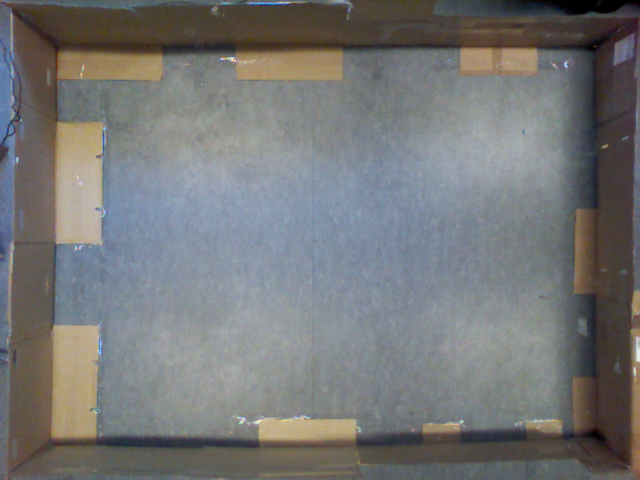
\includegraphics[width=\textwidth]{verden/oppefra}
	\caption{Aktuelt Kørselsmiljø}
	\label{map:world}
	\end{subfigure}
	\begin{subfigure}[b]{.45\textwidth}
	\centering
	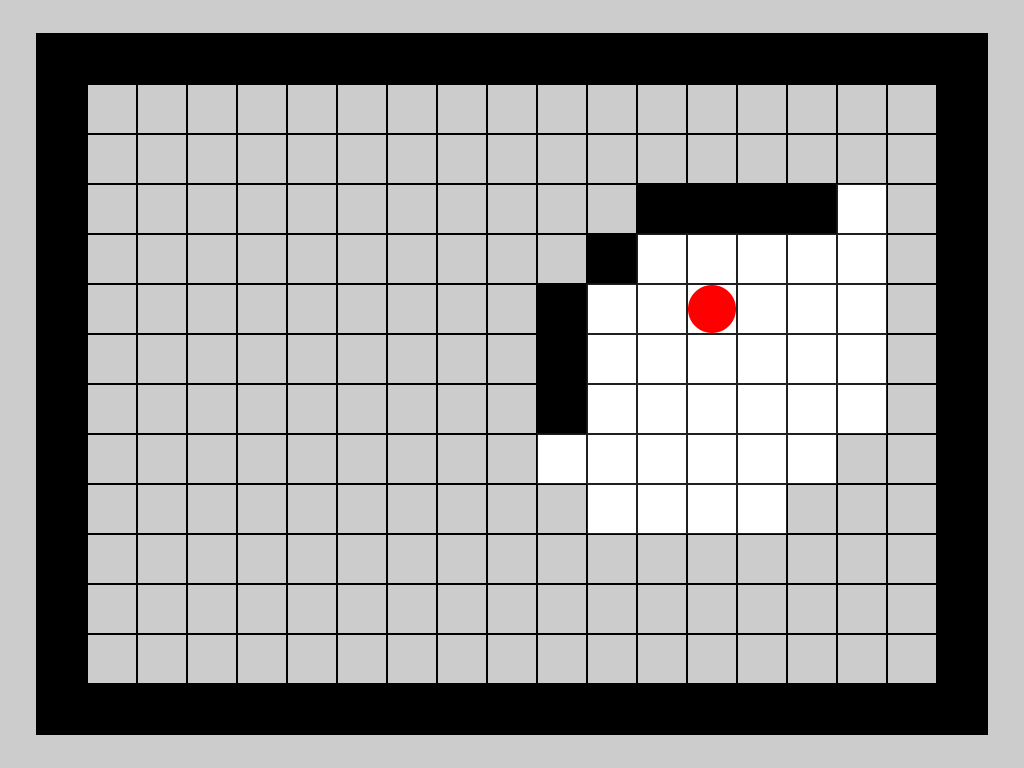
\includegraphics[width=\textwidth]{verden/occupancy_grid_verden}
	\caption{Eksempel på Occupancy Grid}
	\label{map:occupancy_grid}
	\end{subfigure}
\caption{Illustration af et occupancy grid baseret på projekts kørselsmiljø for robotten. Sorte celler i \cref{map:occupancy_grid} indikerer at $\mathcal{P}(occupied) = 1$, hvilket betegner væggene i kørselsmiljøet (\cref{map:world}). Hvide celler indikerer at $\mathcal{P}(occupied) = 0$ og grå celler angiver ikke-udforsket område. Den røde cirkel indikerer robottens position.}
\label{map:approx_occupancy_grid}
\end{figure}

\section{Vertikal og horisontal sensor model}\label{mapping:sensormodel}
Hvis vi antager, at alle objekter i opstillingen er placeret vinkelret til områdets x og y akser,
kan vi konstruere en forholdsvis simpel basal sensormodel.
Først beregner vi afstanden fra robotten til den pågældende celle i vores occupancy grid.

\begin{equation}
r = \mid x_{cell} - x_{robot} + y_{cell} - y_{robot} \mid
\end{equation}

Sensormodellen tildeler de celler, som ligger tæt på den målte afstand fra robotten $z_t$ en højere værdi, kaldet $l_{occ}$, end den prior \textit{belief} $l_0$ fra \cref{eqn:l0}.
De celler som ligger imellem robotten og sensormålingen, tildeles en lavere værdi end $l_0$, kaldet $l_{free}$. 

for at komme frem til hvad tæt på $z_t$ er, indfører vi en konstant $\alpha$ som repræsentere den gennemsnitslige tykkelse af objekter i området.

Sandsynligheden for at cellen er \emph{occupied}, kaldet $l_r$, tildeles således.

\begin{equation}
l_{r} = \begin{cases} 
	l_0 &\text{hvis }r > \text{min}(z_{max},z_t+\frac{\alpha}{2}) \\ 
	l_{occ} &\text{hvis } z_t-\frac{\alpha}{2} \leq r \leq z_t+\frac{\alpha}{2}\\ 
	l_{free} &\text{ellers}  
\end{cases}
\end{equation} \\
Hvor $z_{max}$ er sensorens maksimale måleafstand.
\\
Modellen vil se således ud beskrevet i pseudokode:

\begin{algorithm}[H]
\textbf{InversSensorModel($m_i, x_t, z_t$)} \\
Let $x_i,y_i$ be the center-of-mass of $m_i$ \\
$r = |x_i - x + y_i - y|$ \\
\If{$r > min(z_{max}, z_t + \frac{\alpha}{2}$)}{
	\Return{$l_0$}
}
\ElseIf{$z_t - \frac{\alpha}{2} \le r \le z + \frac{\alpha}{2}$}{
	\Return{$l_{occ}$}
}
\Else{
	\Return{$l_{free}$}
}
\caption{Invers sensor model algoritme.}
\label{alg:inversesensormodel}
\end{algorithm}

\subsection{Gaussisk sensor model}\label{mapping:gaussisk}

% forklaring af gaussisk støj (central limit theorem)
% tilfældige fejl vil tilnærme sig en gausssisk kurve.
I modellen, beskrevet i det forgående afsnit, antog vi, at en celle
med afstanden $\frac{\alpha}{2}$ fra robottens måling på $z_t$ havde
samme sandsynlighed som en celle med afstanden 0 fra $z_t$.

Hvis vi antager, at de celler som ligger tættere på robottens måling, har en større sandsynlighed for at være \emph{occupied}, end dem som ligger tæt på $z_t \pm \frac{\alpha}{2}$, kan vi konstruere en sensor model med en glidende overgang fra værdien $l_{occ}$ for cellen i $z_t$ til værdierne $l_{free}$ og $l_0$ for cellerne på position $z_t \pm \frac{\alpha}{2}$. 

Da summen af uafhængige fejlmålinger, ifølge \emph{central limit theorem} vil tilnærme sig
den gaussiske normalfordeling. \cite[p. 223]{ArtificialIntelligence}
Vil det være en god approximation for robottens måleusikkerhed.

For at finde en passende normalfordeling skal vi vælge en passende middelværdi og en passende standard afvigelse. 
Vi ved at centrum, dvs. middelværdien, for fordelingen skal være målingen $z_t$.

\begin{figure}
\centering 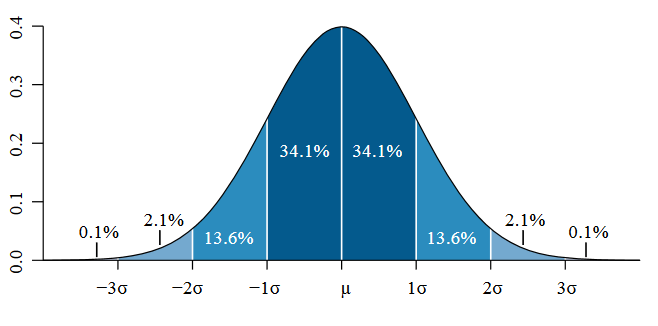
\includegraphics[scale=.75]{NormalDist}
\label{normaldistimg}
\caption{Normal fordeling $\mathcal{N}(\mu,\sigma^2)$}
\end{figure}

Udfra \cref{normaldistimg} kan vi se at det vil være passende hvis $\frac{\alpha}{2}$ svarer til tre standard afvigelser. dvs.
\begin{equation}
	3\sigma = \frac{\alpha}{2} \implies \sigma = \frac{\alpha}{6}
\end{equation}

Vi kan anvende den passende normalfordeling $\mathcal{N}(z_t,\big(\frac{\alpha}{6}\big)^2)$ der ses her. 

\begin{equation}
\mathcal{N}\bigg(z_t,\bigg(\frac{\alpha}{6}\bigg)^2\bigg) = 
\frac{1}{\sqrt{2 \pi \big(\frac{\alpha}{6}\big)^2}}e^{- \frac{(x - z_t)^2}{2 (\frac{\alpha}{6})^2}}
\end{equation}

Vi kan beregne en sandsynlighed, for en celle i afstand $r$, udfra normalfordelingen ved at tage integralet af fordelingen på følgende måde.

\begin{equation}
P(r) = \lim \limits_{\rho \to 0} \bigint_{r-\rho}^{r+\rho} \frac{1}{\sqrt{2 \pi \big(\frac{\alpha}{6}\big)^2}}e^{- \frac{(x - z_t)^2}{2 (\frac{\alpha}{6})^2}}\, \mathrm{d}x
\end{equation}

% Indsæt billede som viser hvorden mapningen vil se ud.

Da vi vil have at sandsynlighederne mellem $z_t-\frac{\alpha}{2}$ og $z_t$ går i en glidende overgang fra $P_{free}$ til $P_{occ}$,
mens vi vil have en overgang fra $P_{occ}$ til ${P_0}$ for afstande imellem $z_t$ og $z_t+\frac{\alpha}{2}$.
Har vi valgt at lave en linær mapning, af de sandsynligheder vi får fra normalfordelingen til de to intervaller, ved hjælp af linjens ligning.
Her er $P_{occ}$,$P_{free}$ og $P_0$ sandsynlighederne for henholdsvis $l_{occ}$,$l_{free}$ og $l_0$.


\begin{equation}
	P_\kappa(r) = \begin{cases}
		\frac{P_{occ}-P_0}{P(z_t)-P(z_t+\frac{\alpha}{2})}(r-P(z_t))+P_{occ} &\text{hvis } z_t < r \\
		\frac{P_{free}-P_{occ}}{P(z_t-\frac{\alpha}{2})-P(z_t)}(r-P(z_t))+P_{occ} &\text{hvis } z_t \leq r 
	\end{cases}
\end{equation}

%######################################

%Da vi vil have, at sandsynligheden i centrum af fordelingen er den samme, som sandsynligheden fra $l_{occ}$ ganger vi med konstanten $\eta$, for på den måde at strække fordelingen så den passer. 

%\begin{equation}
%	P_\eta(r) = \eta P(r) 
%\end{equation}

%For at beregne $\eta$ udfra $l_{occ}$ benytter vi os af \cref{logodds:bel}.

%\begin{equation}
%	\eta P(r) = 1 - \frac{1}{1+e^{l_{occ}}} \implies \eta = \frac{1-\frac{1}{1+e^{l_{occ}}}}{P(r)}
%\end{equation}

%########################################

%\begin{equation}
%	\begin{split}
%		&\eta \lim \limits_{\rho \to 0} \bigint_{z_t-\rho}^{z_t+\rho} \frac{1}{\sqrt{2 \pi \big(\frac{\alpha}{6}\big)^2}}e^{- \frac{(x - z_t)^2}{2 (\frac{\alpha}{6})^2}}\, \mathrm{d}x = 1 - \frac{1}{1+e^{l_{occ}}} \\ 
%	&\implies \eta = \frac{1 - \frac{1}{1+e^{l_{occ}}}}{\lim \limits_{\rho \to 0} \bigint_{z_t-\rho}^{z_t+\rho} \frac{1}{\sqrt{2 \pi \big(\frac{\alpha}{6}\big)^2}}e^{- \frac{(x - z_t)^2}{2 (\frac{\alpha}{6})^2}}\, \mathrm{d}x}
%	\end{split}
%\end{equation}

Den nye tildeling af sandsynlighed til cellen vil nu se således ud.

%\begin{equation}
%	l_{r} = \begin{cases} 
%		l_0 &\text{hvis }r > \text{min}(z_{max},z_t+\frac{\alpha}{2}) \\
%		max\Bigg(l_{0},log\Big(\frac{P_\eta(r)}{1-P_\eta(r)}\Big)\Bigg) &\text{hvis } z_t < r \leq z_t+\frac{\alpha}{2} \\
%		max\Bigg(l_{free},log\Big(\frac{P_\eta(r)}{1-P_\eta(r)}\Big)\Bigg) &\text{hvis } z_t-\frac{\alpha}{2} \leq r \leq z_t \\
%		l_{free} &\text{ellers}	
%	\end{cases} 
%\end{equation}
%Hvor $l_0$ er defineret i \cref{eqn:l0} og $z_{max}$ er sensorens maksimale måleafstand.

\begin{equation}
	l_{r} = \begin{cases} 
		l_0 &\text{hvis }r > \text{min}(z_{max},z_t+\frac{\alpha}{2}) \\
		log\Big(\frac{P_\kappa(r)}{1-P_\kappa(r)}\Big) &\text{hvis } z_t < r \leq z_t+\frac{\alpha}{2} \\
		log\Big(\frac{P_\kappa(r)}{1-P_\kappa(r)}\Big) &\text{hvis } z_t-\frac{\alpha}{2} \leq r \leq z_t \\
		l_{free} &\text{ellers}	
	\end{cases} 
\end{equation}
Hvor $l_0$ er defineret i \cref{eqn:l0} og $z_{max}$ er sensorens maksimale måleafstand.



%
%\subsection{Generel udgave af sensor modellen}
%
%% objekter kan placeres i alle vinkler
%
%\subsubsection{Generel model med gaussisk støj}
%
%% gaussisk støj i 2-d
%
%
%\subsection{tilpasset sensor model}
%
%
%% overfitting
%
%\subsection{sensor model baseret på målinger}
%
%% fejl i sensor er ikke nødvendigvis 'tilfældige' eller uafhængige
%% en generel sensormodel som benytter en sandsynlighedsdistribution som vi selv har målt.
%
%
%\subsection{data udledet udfra robottens placering}
%
%% forbedring hvor vi tager højde for robotten
%
%
%\section{Forward Sensor Model	}
%
%
%














\
